\subsection{Question 1}
We consider $\mathcal{H}_+$ to be the class of positive circles in $\mathbb{R}^2$, and wish to determine the VC-dimension of of $\mathcal{H}_+$. The VC-dimension of a hypothesis set $\mathcal{H}$ is the largest value of $N$ for which $m_{\mathcal{H}}(N)=2^N$.
 	So in short we want to find the largest numbers of points we can shatter/classify by $h \in \mathcal{H}_+$.

Well 2 points is obviously possible to shatter.
More interesting are 3 points for which I created a figure to show all possible triangle arrangements $2^3$ arrangements:

\begin{figure}[!htb]
	\center
	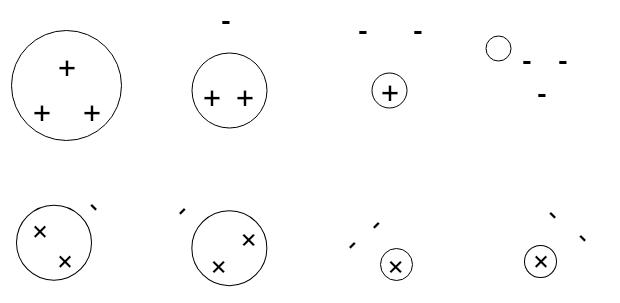
\includegraphics[width=\textwidth]{vc_dimension/vc-dimension}
	\caption{shattering 3 points}
\end{figure}

So we now we would need to shatter 4 points, which is not in all cases possible, following a working case and a not working case:

\begin{figure}[!htb]
		\center
	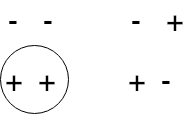
\includegraphics[width=0.5\textwidth]{vc_dimension/vc-dimension-2}
	\caption{shattering 4 points}
\end{figure}

So here the right case wouldn't be possible to shatter with a circle.
So therefore we need to have: $d_{\text{VC}}(\mathcal{H}_+)=3$.
\subsection{Question 2}
In this question we consider $\mathcal{H}= \mathcal{H}_+ \cup \mathcal{H}_-$, where $\mathcal{H}_-$ denotes negative circles in $\mathbb{R}^2$. 
In this case we are able to find examples which actually work with shattered 4 points:

\begin{figure}[!htb]
	\center
	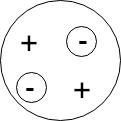
\includegraphics[width=0.3\textwidth]{vc_dimension/vc-dimension-3.png}
	\caption{shattering 4 points}
\end{figure}
So now we can draw negative circles around negatives, since the negative circles are positive on the outside.
This way we can say $d_{\text{VC}}(\mathcal{H})=4$, for all points more than 4 probably can also be shown that it would be possible but I only proved it for 4 now.   